\documentclass[]{article}
\usepackage{lmodern}
\usepackage{amssymb,amsmath}
\usepackage{ifxetex,ifluatex}
\usepackage{fixltx2e} % provides \textsubscript
\ifnum 0\ifxetex 1\fi\ifluatex 1\fi=0 % if pdftex
  \usepackage[T1]{fontenc}
  \usepackage[utf8]{inputenc}
\else % if luatex or xelatex
  \ifxetex
    \usepackage{mathspec}
    \usepackage{xltxtra,xunicode}
  \else
    \usepackage{fontspec}
  \fi
  \defaultfontfeatures{Mapping=tex-text,Scale=MatchLowercase}
  \newcommand{\euro}{€}
\fi
% use upquote if available, for straight quotes in verbatim environments
\IfFileExists{upquote.sty}{\usepackage{upquote}}{}
% use microtype if available
\IfFileExists{microtype.sty}{%
\usepackage{microtype}
\UseMicrotypeSet[protrusion]{basicmath} % disable protrusion for tt fonts
}{}
\usepackage[margin=1in]{geometry}
\usepackage{color}
\usepackage{fancyvrb}
\newcommand{\VerbBar}{|}
\newcommand{\VERB}{\Verb[commandchars=\\\{\}]}
\DefineVerbatimEnvironment{Highlighting}{Verbatim}{commandchars=\\\{\}}
% Add ',fontsize=\small' for more characters per line
\usepackage{framed}
\definecolor{shadecolor}{RGB}{248,248,248}
\newenvironment{Shaded}{\begin{snugshade}}{\end{snugshade}}
\newcommand{\KeywordTok}[1]{\textcolor[rgb]{0.13,0.29,0.53}{\textbf{{#1}}}}
\newcommand{\DataTypeTok}[1]{\textcolor[rgb]{0.13,0.29,0.53}{{#1}}}
\newcommand{\DecValTok}[1]{\textcolor[rgb]{0.00,0.00,0.81}{{#1}}}
\newcommand{\BaseNTok}[1]{\textcolor[rgb]{0.00,0.00,0.81}{{#1}}}
\newcommand{\FloatTok}[1]{\textcolor[rgb]{0.00,0.00,0.81}{{#1}}}
\newcommand{\CharTok}[1]{\textcolor[rgb]{0.31,0.60,0.02}{{#1}}}
\newcommand{\StringTok}[1]{\textcolor[rgb]{0.31,0.60,0.02}{{#1}}}
\newcommand{\CommentTok}[1]{\textcolor[rgb]{0.56,0.35,0.01}{\textit{{#1}}}}
\newcommand{\OtherTok}[1]{\textcolor[rgb]{0.56,0.35,0.01}{{#1}}}
\newcommand{\AlertTok}[1]{\textcolor[rgb]{0.94,0.16,0.16}{{#1}}}
\newcommand{\FunctionTok}[1]{\textcolor[rgb]{0.00,0.00,0.00}{{#1}}}
\newcommand{\RegionMarkerTok}[1]{{#1}}
\newcommand{\ErrorTok}[1]{\textbf{{#1}}}
\newcommand{\NormalTok}[1]{{#1}}
\usepackage{graphicx}
\makeatletter
\def\maxwidth{\ifdim\Gin@nat@width>\linewidth\linewidth\else\Gin@nat@width\fi}
\def\maxheight{\ifdim\Gin@nat@height>\textheight\textheight\else\Gin@nat@height\fi}
\makeatother
% Scale images if necessary, so that they will not overflow the page
% margins by default, and it is still possible to overwrite the defaults
% using explicit options in \includegraphics[width, height, ...]{}
\setkeys{Gin}{width=\maxwidth,height=\maxheight,keepaspectratio}
\ifxetex
  \usepackage[setpagesize=false, % page size defined by xetex
              unicode=false, % unicode breaks when used with xetex
              xetex]{hyperref}
\else
  \usepackage[unicode=true]{hyperref}
\fi
\hypersetup{breaklinks=true,
            bookmarks=true,
            pdfauthor={Benjamin Weigel},
            pdftitle={WEB272 -- SOMT Refolding},
            colorlinks=true,
            citecolor=blue,
            urlcolor=blue,
            linkcolor=magenta,
            pdfborder={0 0 0}}
\urlstyle{same}  % don't use monospace font for urls
\setlength{\parindent}{0pt}
\setlength{\parskip}{6pt plus 2pt minus 1pt}
\setlength{\emergencystretch}{3em}  % prevent overfull lines
\setcounter{secnumdepth}{5}

%%% Use protect on footnotes to avoid problems with footnotes in titles
\let\rmarkdownfootnote\footnote%
\def\footnote{\protect\rmarkdownfootnote}

%%% Change title format to be more compact
\usepackage{titling}

% Create subtitle command for use in maketitle
\newcommand{\subtitle}[1]{
  \posttitle{
    \begin{center}\large#1\end{center}
    }
}

\setlength{\droptitle}{-2em}
  \title{WEB272 -- SOMT Refolding}
  \pretitle{\vspace{\droptitle}\centering\huge}
  \posttitle{\par}
  \author{Benjamin Weigel}
  \preauthor{\centering\large\emph}
  \postauthor{\par}
  \predate{\centering\large\emph}
  \postdate{\par}
  \date{07/23/2015}



\begin{document}

\maketitle


{
\hypersetup{linkcolor=black}
\setcounter{tocdepth}{2}
\tableofcontents
}
After rebuffering protein concentrations were measured by Bradford:

\section{Protein concetration}\label{protein-concetration}

\includegraphics{analysis_files/figure-latex/unnamed-chunk-2-1.pdf}

\subsection{Regression tree}\label{regression-tree}

Next we build a regression tree. To see, which factors have the most
influence on the protein concentration.

\begin{Shaded}
\begin{Highlighting}[]
\NormalTok{somttree2 <-}\StringTok{ }\KeywordTok{rpart}\NormalTok{(BFmean ~}\StringTok{ }\NormalTok{., }
                \DataTypeTok{data=}\NormalTok{df[,}\KeywordTok{c}\NormalTok{(}\DecValTok{1}\NormalTok{:}\DecValTok{11}\NormalTok{,}\DecValTok{21}\NormalTok{)],}
                \DataTypeTok{control =} \KeywordTok{c}\NormalTok{(}\DataTypeTok{minsplit =} \DecValTok{3}\NormalTok{,}
                            \DataTypeTok{minbucket =} \DecValTok{2}\NormalTok{,}
                            \DataTypeTok{complexity =} \FloatTok{0.001}\NormalTok{))}
\KeywordTok{fancyRpartPlot}\NormalTok{(somttree2, }\DataTypeTok{digits=}\DecValTok{3}\NormalTok{)}
\end{Highlighting}
\end{Shaded}

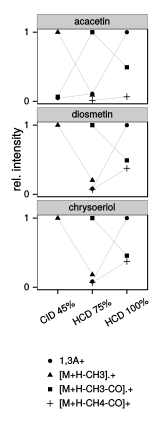
\includegraphics{analysis_files/figure-latex/unnamed-chunk-3-1.pdf}

Arginine seems to have the biggest impact on refolding efficiency
(Arginine addition is better). Then comes SAH (no SAH is better).

\subsection{Main effects plot}\label{main-effects-plot}

\includegraphics{analysis_files/figure-latex/unnamed-chunk-4-1.pdf}

\begin{verbatim}
## % latex table generated in R 3.1.2 by xtable 1.7-4 package
## % Thu Oct 22 11:41:42 2015
## \begin{table}[ht]
## \centering
## \begin{tabular}{rllr}
##   \hline
##  & state & ME & value \\ 
##   \hline
## 1 & - & pH & 11.34 \\ 
##   2 & + & pH & 24.63 \\ 
##   3 & - & Arginine & 0.67 \\ 
##   4 & + & Arginine & 35.29 \\ 
##   5 & - & Glycerin & 25.90 \\ 
##   6 & + & Glycerin & 10.07 \\ 
##   7 & - & ionicStrength & 15.36 \\ 
##   8 & + & ionicStrength & 20.60 \\ 
##   9 & - & divCations & 18.66 \\ 
##   10 & + & divCations & 17.30 \\ 
##   11 & - & redox & 18.66 \\ 
##   12 & + & redox & 17.30 \\ 
##   13 & - & CycloDex & 14.63 \\ 
##   14 & + & CycloDex & 21.33 \\ 
##   15 & - & SAH & 26.63 \\ 
##   16 & + & SAH & 9.34 \\ 
##    \hline
## \end{tabular}
## \end{table}
\end{verbatim}

\includegraphics{analysis_files/figure-latex/unnamed-chunk-5-1.pdf}

\subsection{Statistical test}\label{statistical-test}

Test the statistical significance of main effects. Only Arginine is
statistically significant to a p-value of 0.05. SAH to a p-value of 0.1.

\% latex table generated in R 3.1.2 by xtable 1.7-4 package \% Thu Oct
22 11:41:44 2015

\begin{table}[ht]
\centering
\begin{tabular}{lrrrrr}
  \hline
 & Df & Sum Sq & Mean Sq & F value & Pr($>$F) \\ 
  \hline
Arginine      & 1 & 3595.63 & 3595.63 & 24.56 & 0.0158 \\ 
  pH            & 1 & 529.87 & 529.87 & 3.62 & 0.1533 \\ 
  Glycerin      & 1 & 752.08 & 752.08 & 5.14 & 0.1083 \\ 
  ionicStrength & 1 & 82.37 & 82.37 & 0.56 & 0.5077 \\ 
  divCations    & 1 & 5.49 & 5.49 & 0.04 & 0.8588 \\ 
  redox         & 1 & 5.52 & 5.52 & 0.04 & 0.8584 \\ 
  CycloDex      & 1 & 134.67 & 134.67 & 0.92 & 0.4083 \\ 
  SAH           & 1 & 896.83 & 896.83 & 6.13 & 0.0897 \\ 
  Residuals     & 3 & 439.26 & 146.42 &  &  \\ 
   \hline
\end{tabular}
\end{table}

\begin{verbatim}
## Error in eval(expr, envir, enclos): could not find function "LenthPlot"
\end{verbatim}

\section{Protein volume activity}\label{protein-volume-activity}

\includegraphics{analysis_files/figure-latex/unnamed-chunk-7-1.pdf}
\includegraphics{analysis_files/figure-latex/unnamed-chunk-7-2.pdf}

\subsection{Regression tree}\label{regression-tree-1}

Next we build a regression tree. To see, which factors have the most
influence the SOMT activity.

\begin{Shaded}
\begin{Highlighting}[]
\NormalTok{somttree2 <-}\StringTok{ }\KeywordTok{rpart}\NormalTok{(P1_AC ~}\StringTok{ }\NormalTok{., }
                \DataTypeTok{data=}\NormalTok{df[,}\KeywordTok{c}\NormalTok{(}\DecValTok{1}\NormalTok{:}\DecValTok{8}\NormalTok{,}\DecValTok{12}\NormalTok{)],}
                \DataTypeTok{control =} \KeywordTok{c}\NormalTok{(}\DataTypeTok{minsplit =} \DecValTok{3}\NormalTok{,}
                            \DataTypeTok{minbucket =} \DecValTok{2}\NormalTok{,}
                            \DataTypeTok{complexity =} \FloatTok{0.001}\NormalTok{))}
\KeywordTok{fancyRpartPlot}\NormalTok{(somttree2, }\DataTypeTok{digits=}\DecValTok{3}\NormalTok{)}
\end{Highlighting}
\end{Shaded}

\includegraphics{analysis_files/figure-latex/unnamed-chunk-8-1.pdf}

The redox status seems to have the biggest impact on refolding
efficiency measured by activity (reducing is better, DTT). Then comes
arginine (arginine is better).

\subsection{Main effects plot}\label{main-effects-plot-1}

\subsubsection{ÁUC}\label{auc}

\includegraphics{analysis_files/figure-latex/unnamed-chunk-9-1.pdf}

\includegraphics{analysis_files/figure-latex/unnamed-chunk-10-1.pdf}

\subsubsection{conversion}\label{conversion}

\includegraphics{analysis_files/figure-latex/unnamed-chunk-11-1.pdf}

\includegraphics{analysis_files/figure-latex/unnamed-chunk-12-1.pdf}

\subsection{Statistical test}\label{statistical-test-1}

Test the statistical significance of main effects. Only Arginine is
statistically significant to a p-value of 0.05. SAH to a p-value of 0.1.

\subsubsection{AUC}\label{auc-1}

\% latex table generated in R 3.1.2 by xtable 1.7-4 package \% Thu Oct
22 11:41:50 2015

\begin{table}[ht]
\centering
\begin{tabular}{lrrrrr}
  \hline
 & Df & Sum Sq & Mean Sq & F value & Pr($>$F) \\ 
  \hline
pH            & 1 & 0.02 & 0.02 & 4.83 & 0.1153 \\ 
  Arginine      & 1 & 0.03 & 0.03 & 8.14 & 0.0649 \\ 
  Glycerin      & 1 & 0.00 & 0.00 & 0.55 & 0.5122 \\ 
  ionicStrength & 1 & 0.01 & 0.01 & 3.27 & 0.1682 \\ 
  divCations    & 1 & 0.00 & 0.00 & 0.57 & 0.5047 \\ 
  redox         & 1 & 0.06 & 0.06 & 19.88 & 0.0210 \\ 
  CycloDex      & 1 & 0.00 & 0.00 & 0.78 & 0.4428 \\ 
  SAH           & 1 & 0.00 & 0.00 & 0.13 & 0.7439 \\ 
  Residuals     & 3 & 0.01 & 0.00 &  &  \\ 
   \hline
\end{tabular}
\end{table}

\includegraphics{analysis_files/figure-latex/unnamed-chunk-13-1.pdf}
alpha PSE ME SME 0.05000000 0.03975856 0.11446004 0.24518392

\subsubsection{conversion}\label{conversion-1}

\% latex table generated in R 3.1.2 by xtable 1.7-4 package \% Thu Oct
22 11:41:50 2015

\begin{table}[ht]
\centering
\begin{tabular}{lrrrrr}
  \hline
 & Df & Sum Sq & Mean Sq & F value & Pr($>$F) \\ 
  \hline
pH            & 1 & 5.71 & 5.71 & 4.55 & 0.1227 \\ 
  Arginine      & 1 & 8.31 & 8.31 & 6.62 & 0.0824 \\ 
  Glycerin      & 1 & 0.44 & 0.44 & 0.35 & 0.5945 \\ 
  ionicStrength & 1 & 3.38 & 3.38 & 2.69 & 0.1997 \\ 
  divCations    & 1 & 0.54 & 0.54 & 0.43 & 0.5605 \\ 
  redox         & 1 & 24.26 & 24.26 & 19.31 & 0.0218 \\ 
  CycloDex      & 1 & 1.07 & 1.07 & 0.85 & 0.4250 \\ 
  SAH           & 1 & 0.11 & 0.11 & 0.09 & 0.7893 \\ 
  Residuals     & 3 & 3.77 & 1.26 &  &  \\ 
   \hline
\end{tabular}
\end{table}

\includegraphics{analysis_files/figure-latex/unnamed-chunk-14-1.pdf}
alpha PSE ME SME 0.0500000 0.7637776 2.1988227 4.7100805

\end{document}
